
\definecolor{grey}{RGB}{128,128,128}


\def \globalscale {0.90000}
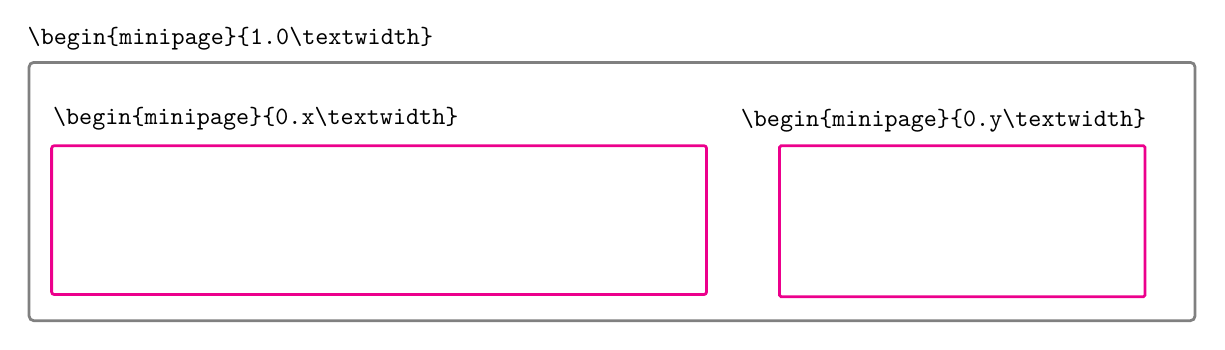
\begin{tikzpicture}[y=1pt, x=1pt, yscale=-\globalscale,xscale=\globalscale, every node/.append style={scale=\globalscale}, inner sep=0pt, outer sep=0pt]
  \begin{scope}[shift={(-13.79, -47.88)}]
    \path[draw=grey,fill opacity=1.0,line width=1.0pt,rounded corners=1.71pt] 
  (69.34, 253.29) rectangle (537.49, 357.0);



    \path[draw=magenta,fill opacity=1.0,line width=1.0pt,rounded corners=0.96pt]
   (78.4, 286.74) rectangle (341.36, 346.51);



    \path[draw=magenta,fill opacity=1.0,line width=1.0pt,rounded corners=0.54pt]
   (370.65, 286.79) rectangle (517.42, 347.35);



    \node[text=black,line width=3.98pt,anchor=south west] (text1) at (68.81, 
  248.52){\verb+\begin{minipage}{1.0\textwidth}+};



    \node[text=black,line width=3.98pt,anchor=south west] (text1-5) at (355.11, 
  281.3){\verb+\begin{minipage}{0.y\textwidth}+};



    \node[text=black,line width=3.98pt,anchor=south west] (text1-5-2) at (78.98,
   280.49){\verb+\begin{minipage}{0.x\textwidth}+};



  \end{scope}

\end{tikzpicture}
